% !TEX root = Zusammenfassung.tex
\chapter{Spezifikation}

\section{Abstraktion: Episch reflektive Subkategorien}

\paragraph{\defi 152: Subkategorie}
Kategorie $\mathcal{D}$ ist Subkategorie von $\mathcal{C}$ ($\mathcal{D} \subseteq \mathcal{C}$), wenn
\begin{enumerate}
\item $O^\mathcal{D} \subseteq O^\mathcal{C}$ (Objekte in Teilmengenbeziehung)
\item $\forall \, a,b \in O^\mathcal{D}:  M^\mathcal{D}_{a,b} \subseteq M^\mathcal{C}_{a,b} $
\item $\forall \, a \in O^\mathcal{D}: id^\mathcal{D}_a = id^\mathcal{C}_a$
\item $\forall \, a,b,c, \in O^\mathcal{D} \wedge m \in M^\mathcal{D}_{a,b}, n \in M^\mathcal{D}_{b,c}: n \circ^{\mathcal{D}}_{a,b,c} m  = n \circ^{\mathcal{C}}_{a,b,c} m  $
\end{enumerate}

\begin{itemize}
\item $\mathcal{D}$ ist voll, wenn
\begin{enumerate}
\item $\mathcal{D} \subseteq \mathcal{C}$ und
\item $\forall \, a,b \in O^\mathcal{D}:  M^\mathcal{D}_{a,b} = M^\mathcal{C}_{a,b} $
\end{enumerate}
\item $\mathcal{D}$ ist isomorph geschlossen, wenn $\approx: a \rightarrow b \in M^\mathcal{C}_{a,b} \text{ mit } a \in O^\mathcal{D} \implies b \in O^\mathcal{D}$
\item Wenn $\mathcal{D}$ voll und isomorph-geschlossen ist: $\mathcal{D} \subseteq^{\approx} \mathcal{C}$
\end{itemize}

Notiz: Nur isomorph-geschlossene Kategorien sind abstrakt (bis auf Isomorphie)!

\paragraph{\defi 153: Episch reflektive Subkategorie}
$\mathcal{D}$ ist reflektive Subkategorie von $\mathcal{C}$, wenn
\begin{enumerate}
\item $\mathcal{D} \subseteq \mathcal{C}$
\item $\forall \, c \in O^\mathcal{C}: $  gibt es 
\begin{itemize}
\item ein $c_\mathcal{D} $ ($\mathcal{D}$- Reflektion von $c$) und 
\item ein Morphismus $\eta_c: c \rightarrow c_\mathcal{D} $ (Reflektor von $c$) 
\end{itemize}
\end{enumerate}

mit der folgenden Eigenschaft: $\forall \,  m: c \rightarrow z$, so dass $z \in \mathcal{D}$, dann gibt es einen eindeutigen Morphismus $m^* : c_\mathcal{D} \rightarrow z$ mit $m^* \circ \eta = m$ \\
$\mathcal{D} $ ist episch reflektiv, wenn zusätzlich alle Reflektoren epis sind. 

\begin{figure}[h]
\noindent \centering{}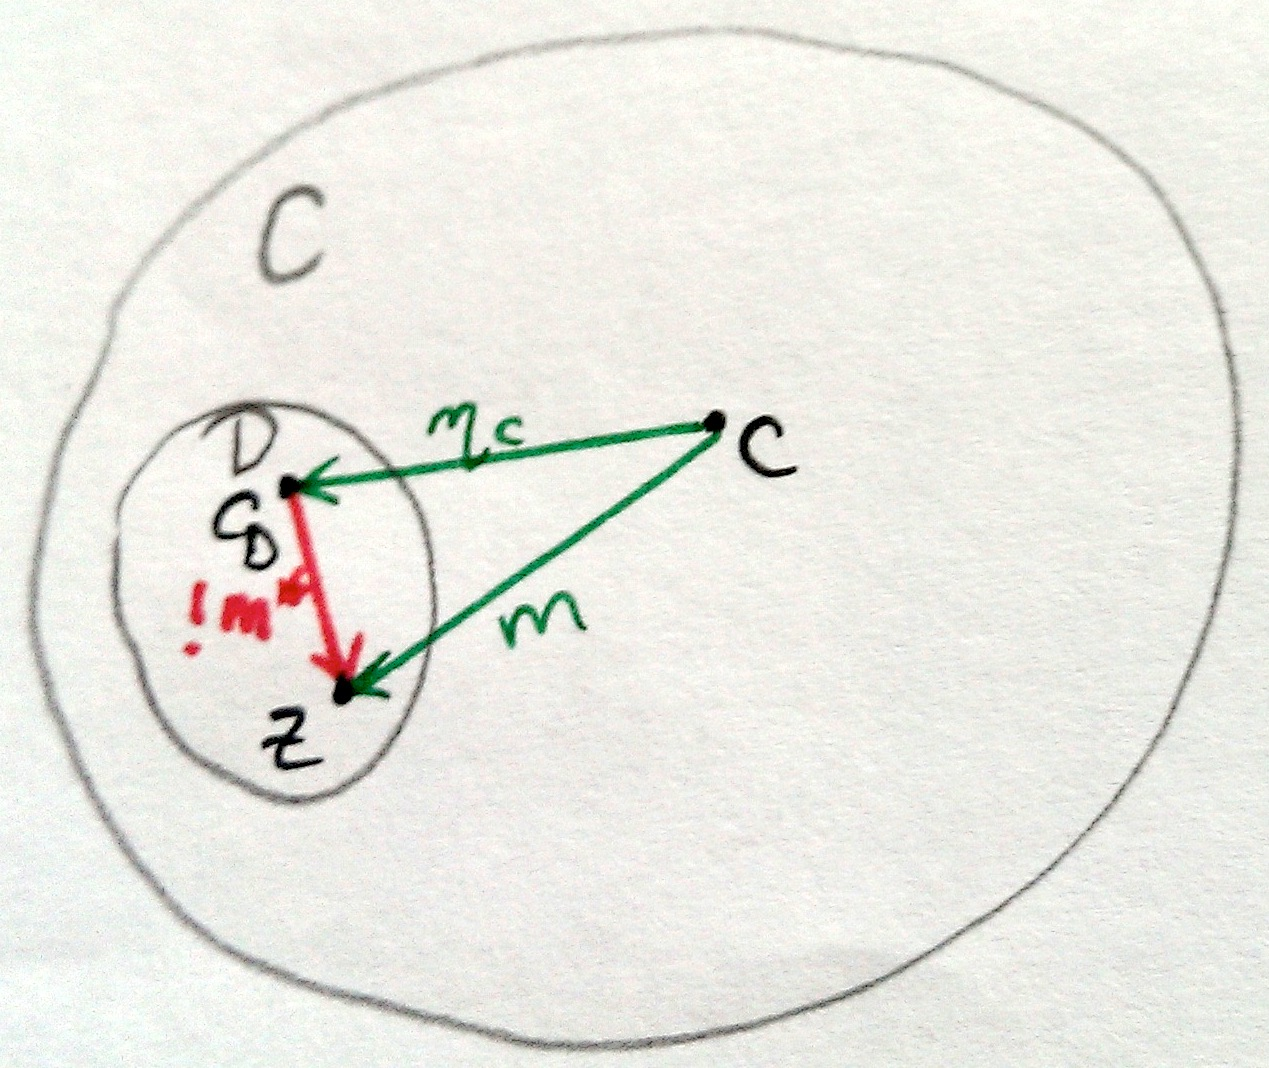
\includegraphics[scale=0.1]{Abbildungen/153}\caption{Episch reflektive Subkategorie}
\end{figure}

\paragraph{\prop 154: Reflektionen sind abstrakt}
Sei $\mathcal{D} $ reflektive Subkategorie von $\mathcal{C} $

\begin{enumerate}
\item $\eta_1: c \rightarrow c_\mathcal{D}^1 $ und $\eta_2: c \rightarrow c_\mathcal{D}^2 $ zwei Relfektionen von $\mathcal{C} \implies \approx: \mathcal{C}_\mathcal{D}^1 \rightarrow \mathcal{C}_\mathcal{D}^2 $ mit $\eta: c \rightarrow \mathcal{C}_\mathcal{D}^2$
\item  $\eta: c \rightarrow \mathcal{C}_\mathcal{D}^1$ Reflektor für $c$ und $\approx: c_\mathcal{D}^1 \rightarrow c_\mathcal{D}^2$ ist Iso $\implies \eta' \, = \, \approx \circ \eta : c \rightarrow c_\mathcal{D}^2$ ist auch Reflektor für $c$
\end{enumerate}

\begin{figure}[h]
\noindent \centering{}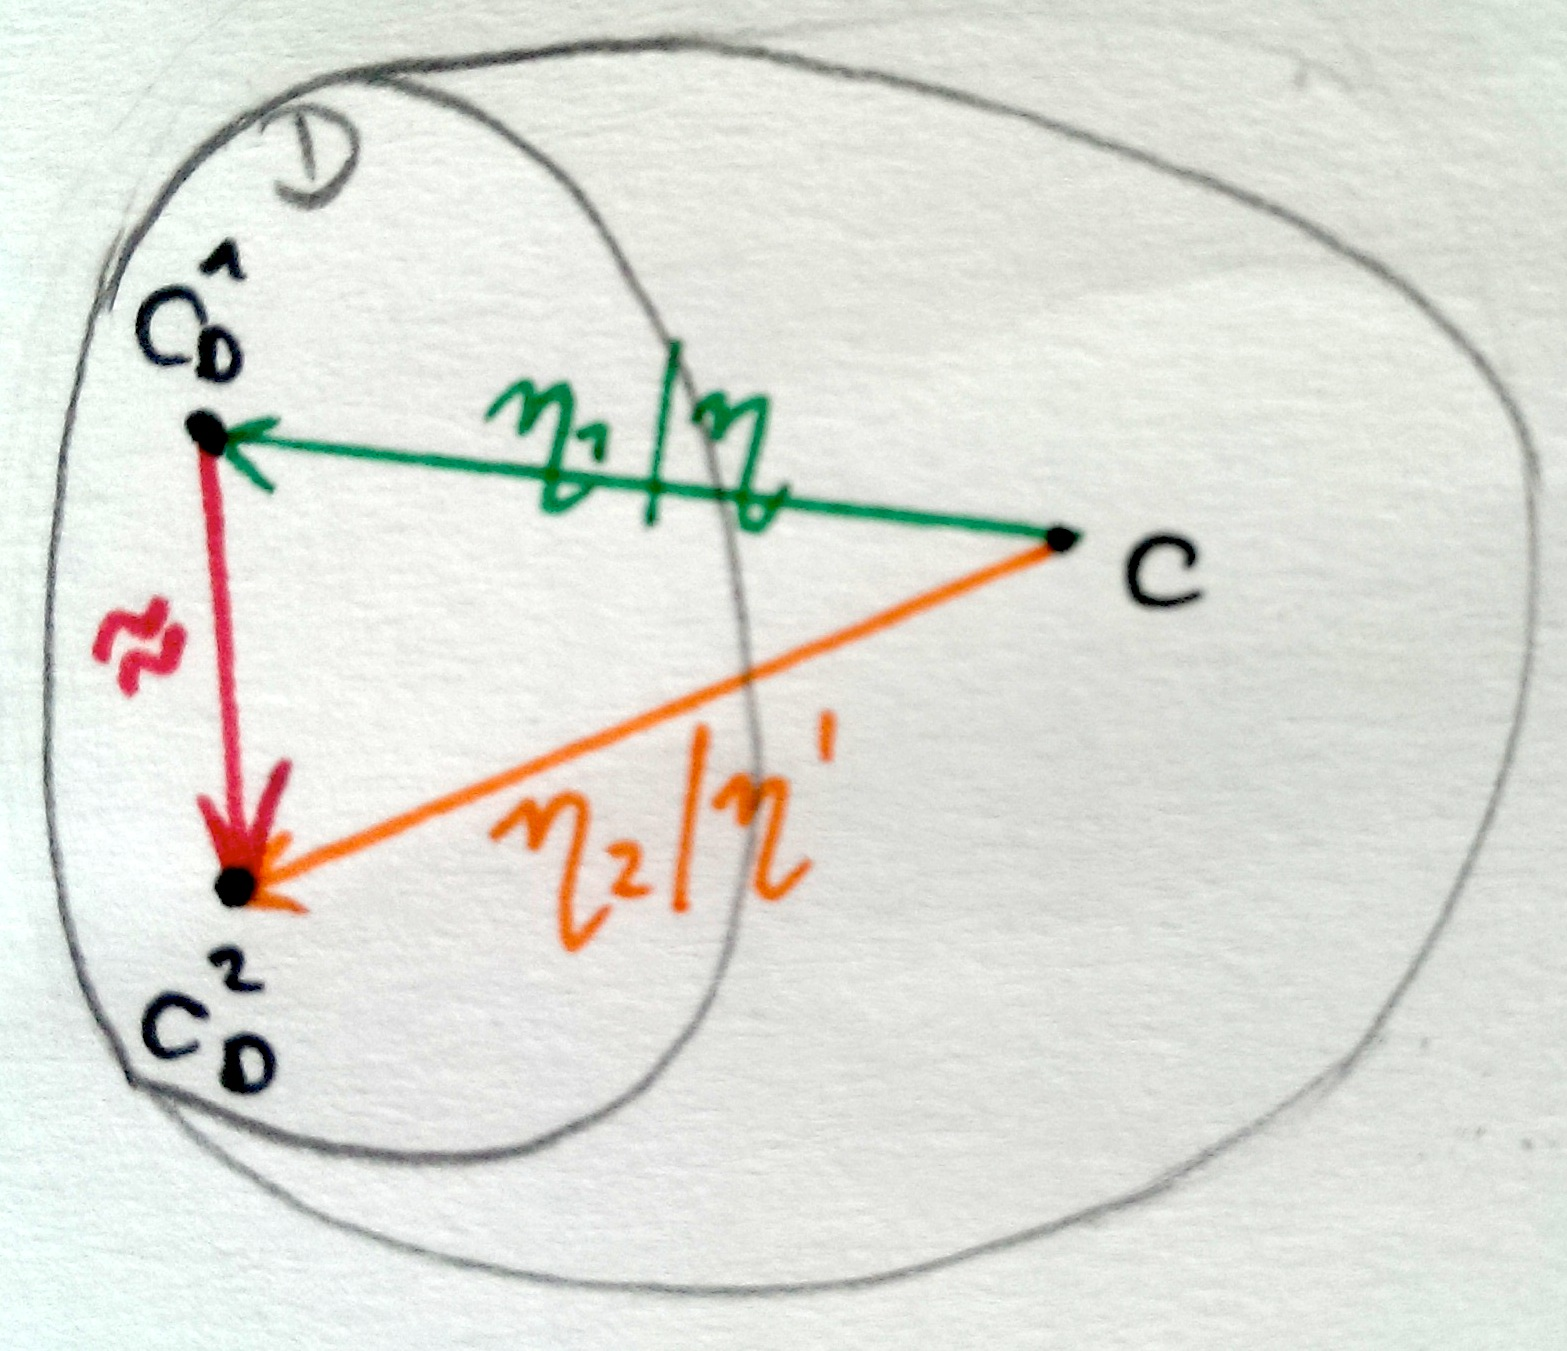
\includegraphics[scale=0.1]{Abbildungen/154}\caption{Reflektionen sind abstrakt}
\end{figure}

\paragraph{\prop 155: Isomorphe Reflektoren}
 
\begin{enumerate}
\item  $\mathcal{D} $ reflektive Subkategorie von $\mathcal{C} $ und $d \in \mathcal{D} \implies \eta_d : d \rightarrow d_\mathcal{D}$ ist iso.
\item  $\mathcal{D} $ ist reflektive und isomorph-geschlossene Subkategorie von $\mathcal{C}$ \\ $ \implies \forall \, c \in \mathcal{C}: c \in \mathcal{D} \Leftrightarrow $ der Reflektor für $c$ ist iso.  
\end{enumerate}

\paragraph{\prop 156: Epische Reflektionen und Produkte}

 $\mathcal{D}$ episch-reflektiv und isomorph-geschlossene Subkategorie von $\mathcal{C}$ und \\ $\Pi \mathcal{A}$ ist Produkt in $\mathcal{C}$ einer Familie $\mathcal{A} = (a_i)_{i \in I} $ von $\mathcal{D}$-Objekten, d.h. $(a_i \in \mathcal{D})_{i \in I}$ \\$ \implies \Pi \mathcal{A} \in \mathcal{D}$
 
 \paragraph{\prop 157: Epische Reflektionen und extremale Monos}
 $\mathcal{D}$ episch-reflektiv und isomorph-geschlossene Subkategorie von $\mathcal{C}$ mit $(\mathcal{E}, \mathcal{M}^x) \implies c \in \mathcal{D}$ wenn $m: c \rightarrowtail d$ ist extremal Mono und $d \in \mathcal{D}$. \\
 D.h. in TCs Worten: \\
 Wenn wir $\mathcal{D}$ aus Def haben und  $(\mathcal{E}, \mathcal{M}^x)$ dann folgt daraus, jedes $d$, was über einen extremalen Mono erreicht wird, hat ein 'Urbild' in $\mathcal{D}$.
 
 
\paragraph{\prop 158: Co-Well-Powered Categories}
Kategorie $\mathcal{C}$ its Co-well-powered, wenn $\forall \, a \in \mathcal{C}$ die 'Collection' abstrakter Quotienten (Def 77) von a eine Menge bildet. \\
\emph{'Colletion abstrakter Quotienten von a' = Paarweise nicht isomorphe Epis mit Domain a.}
 
 
\paragraph{Theorem 159: Charakterisierung episch reflektiver Subkategorien} 
Gegeben: $\mathcal{C}$ co-well-powered Kategorie mit ($\mathcal{E},\mathcal{M}^x$). Isomorph geschlossene Subkategorie $\mathcal{D}$ von $\mathcal{C}$i ist episch reflektiv $\Leftrightarrow \, \mathcal{D} $ geschlossen unter Produkten und extremalen Subobjekten ist. 
 
 
\paragraph{\defi 160 Reflektion von Morphismen}  
Gegeben $\mathcal{D}$ reflektive Subkategorie von $\mathcal{C}$ und $c \mapsto (\eta_c : c \rightarrow c_\mathcal{D})$ eine festgelegte Auswahl von Reflektoren $\eta_c$ für jedes Objekt $c \in \mathcal{C}$.
Dann definieren wir das folgende Mapping von Morphismen $m: c \rightarrow c' \in \mathcal{C}$ zu Morphismen in $\mathcal{D}: m : c \rightarrow c' \mapsto m^\mathcal{D}: c_\mathcal{D} \rightarrow c_\mathcal{D}' \, = \, (\eta_{c'} \circ m)^* : c_\mathcal{D} \rightarrow c_\mathcal{D}'$.  \\
\emph{In CTs Worten: Morphismen werden von $\mathcal{C}$ nach $\mathcal{D}$ reflektiert.}

\begin{figure}[h]
\noindent \centering{}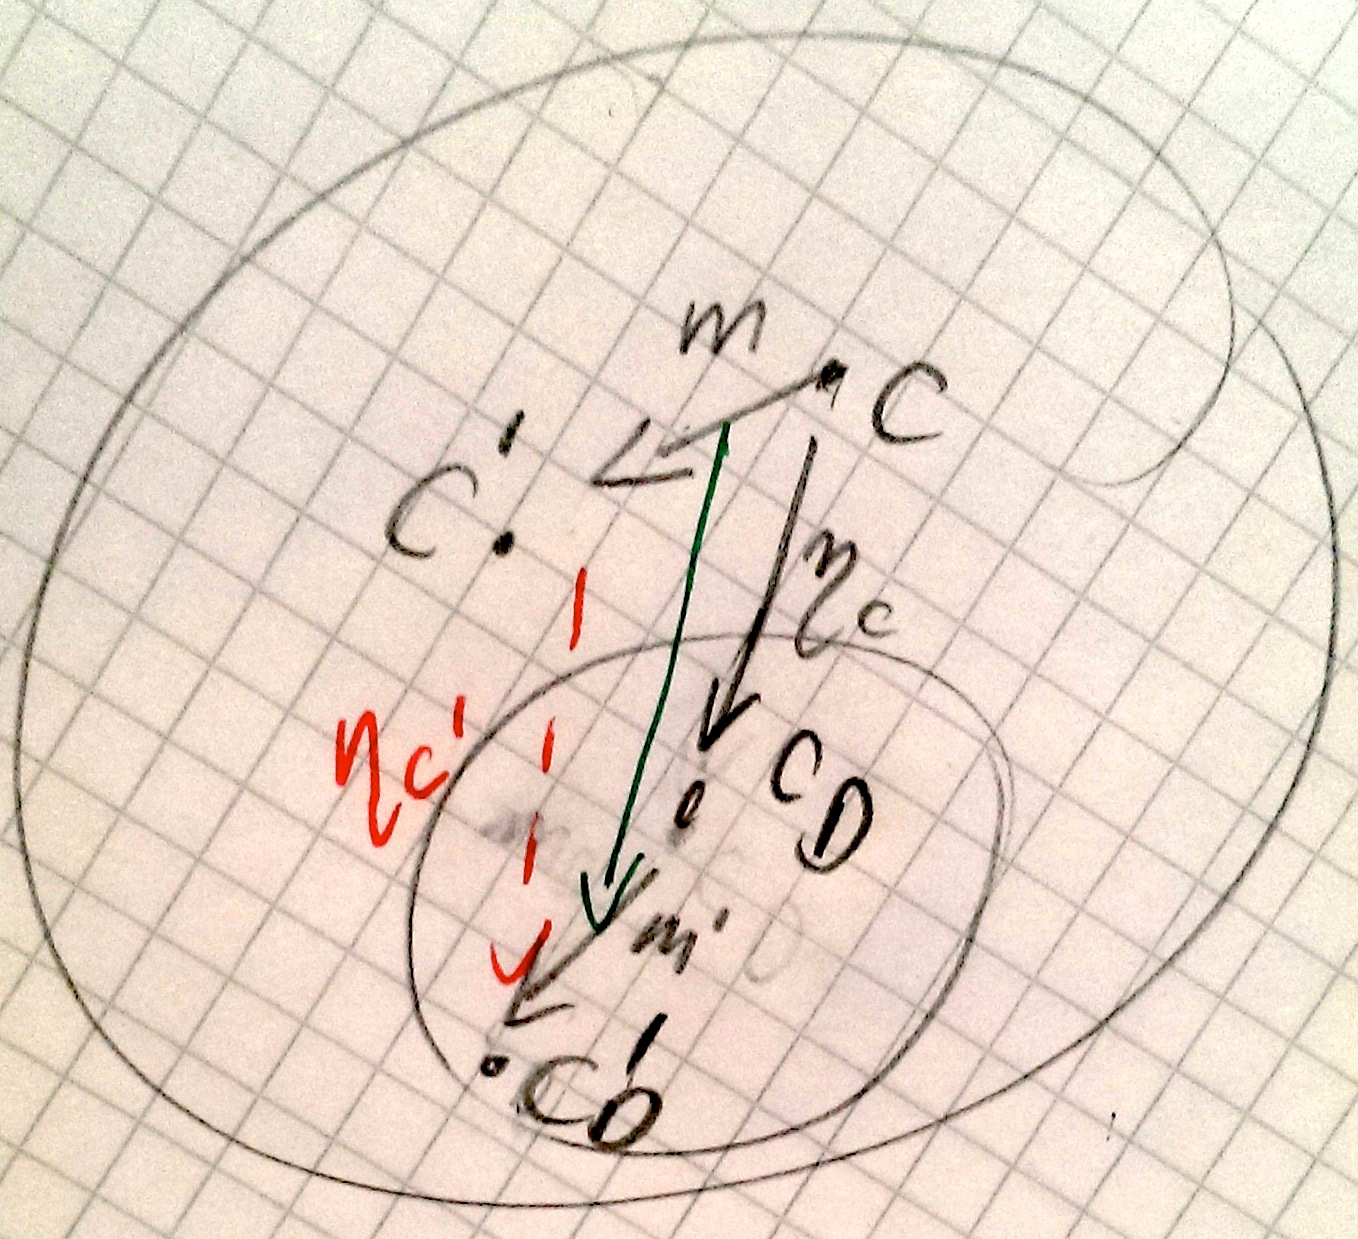
\includegraphics[scale=0.09]{Abbildungen/160}\caption{Reflektion von Monomorphismen}
\end{figure}

\paragraph{\prop 161 Eigenschaften von Morphismusreflektionen}  
$\mathcal{D}$ reflektive Subkategorie von $\mathcal{C}$ und $m \mapsto m^\mathcal{D} \Rightarrow$

\begin{enumerate}
\item $id_c^D = id_{c_\mathcal{D}}$ $\forall c \in C$
\item $(m \circ_\mathcal{C} n)^\mathcal{D} = m^\mathcal{D} \circ_\mathcal{D} n^\mathcal{D}$  wenn $m,n$ komponierbar in $C$.
\end{enumerate}
\emph{CT Notiz zu 2.: Erst verkullern und dann Übertragen ist gleich zu erst einzeln Übertragen und dann verkullern.}


\section{Syntaktifizierung}

\subsection{Terme und Termsysteme}

\paragraph{\defi 162 Variablen-Mengen und Variablen-Systeme}  
Eine Variablenmenge $X$ ist eine S-Indizierte Familie von Mengen von Variablen, d.h. $X = (X_s)_{s \in S*}$ \\
Eine Variablenmenge ist ein algebraisches System in dem alle Funktionen komplett undefiniert sind.

\paragraph{\defi 163 Terme und totale Termsysteme}
Die 'Collection' von Termen $T^{\Sigma,X}$ mit Variablen in $X$ ist die kleinste S-Indizierte Familie von Mengen $T^{\Sigma, X} = (T^{\Sigma, X}_s)_{s \in S}$ die folgende Bedingungen erfüllen:
\begin{enumerate}
\item Variablen: $x \in T^{\Sigma, X}_s $ wenn $x \in X_s$
\item Funktionen: $f_i(t) \in T^{\Sigma, X}_s $ wenn $f \in O_{w,v} $ und $t \in (T^{\Sigma, X})^w $ und $v = v_l sv_r$ und $i = |v_l| +1$

Das totale Termsystem $T^{\Sigma, X}$ mit Variablen in $X$ ist das $\Sigma$-System, welches die Familie von Termen $(T^{\Sigma, X}_s)_{s \in S}$ als Träger nehmen und alle Funktionen definieren durch:

\item Funktionen: Für $f \in O_{w,v} $ und $|v| \geq 1$ und $x \in (T^{\Sigma, X})^w: f^{T^{\Sigma, X}}(x) = (f_i(x))_{i \in 1 \dots |v|}$
\item Prädikate: Für $f \in O_{w, \epsilon}$ und $f \neq \, =: f^{T^{\Sigma, X}} = \emptyset$, d.h. $f^{T^{\Sigma, X}}$ Alle Prädikate bis auf die Gleichheit sind komplett undefiniert. 
\end{enumerate}

\emph{Notiz CT:  1. und 2. definiert die Trägermengen des totalen Termsystems \\
 Zu 3.: Ist das nicht das mit der 'Tiefe' von Termen bei Elsner? s(s(s(...))) \\
'$f \neq =$' bedeutet: f ist nur für = definiert. Sonst nichts}


\paragraph{\defi 164 Operationen auf Termen}  
Die Operationen (a) enthalten Variablen, (b) enthalten Terme und (c) die Höhe ist definiert auf der 'Collection' von Termen $T^{\Sigma, X}$ durch:

1. Fall: Variablen \\
2. Fall: Rekursiver Aufruf für Operationen mit Termen \\
3. Fall: Konstanten \\
4. Fall: Wenn Variable Kreuzprodukt \\

\begin{align*}
\textrm{\_}_{X}:\left(T^{\Sigma,X}\right)^{w}\rightarrow2^{X}\!::=\, & t_{X}=\begin{cases}
\{t\} & t\in X\\
x_{X} & t=f_{i}(x),f\in O_{w,v},1\leq i\leq|v|\\
\emptyset & t\in\left(T^{\Sigma,X}\right)^{\epsilon}\\
x_{X}^{1}\cup x_{X}^{2} & t=x^{1}\times x^{2}
\end{cases} & \textrm{\!(a)}\\
\textrm{\_}_{T}:\left(T^{\Sigma,X}\right)^{w}\rightarrow2^{T^{\Sigma,X}}\!::=\, & t_{T}=\begin{cases}
\{t\} & \! t\in X\\
\{f_{j}(x)::j\in[1,|v|]\}\cup x_{T} & \! t=f_{i}(x),f\in O_{w,v},i\in[1,|v|]\\
\emptyset & \! t\in\left(T^{\Sigma,X}\right)^{\epsilon}\\
x_{T}^{1}\cup x_{T}^{2} & \! t=x^{1}\times x^{2}
\end{cases} & \textrm{\!(b)}\\
|\textrm{\_|:}\left(T^{\Sigma,X}\right)^{w}\rightarrow\mathbb{N}_{0}\!::=\, & |t|=\begin{cases}
0 & t\in X\\
|x|+1 & t=f_{i}(x),f\in O_{w,v},1\leq i\leq|v|\\
0 & t\in\left(T^{\Sigma,X}\right)^{\epsilon}\\
\max(|x^{1}|,|x^{2}|) & t=x^{1}\times x^{2}
\end{cases} & \textrm{\!(c)}
\end{align*}

\paragraph{\defi 165 Partielle Termsysteme}  
Ein partielles Termsystem $P^{\Sigma,X}$ ist ein Subsystem von dem totalen Termsystem $T^{\Sigma,X}$, so dass 
\begin{enumerate}
\item $X \subseteq P^{\Sigma,X}$
\item $\left\lceil X\right\rceil _{P^{\Sigma,X}}^{c}$ (Wenn Argumente des Terms selber wieder Terme sind, sind diese auch in $P^{\Sigma,X}$ enthalten)
\end{enumerate}

\paragraph{\coro 166 Variablen-Einbettung und eindeutiger Homomorphismus}  
\begin{enumerate}
\item Für jedes partielle System $P^{\Sigma,X}$ die Einbettung $X\hookrightarrow P^{\Sigma,X}$ ist epi.
\item $h^1, h^2: P^{\Sigma,X} \rightarrow A$ homo eines partiellen Systems $P^{\Sigma,X}$ in ein anderes algebraisches System $A \implies h_{|X|}^1 = h_{|X|}^2 \implies h^1 = h^2$, d.h. wenn die Homos $h_1$ und $h_2$ in den Variablen übereinstimmen, sind sie gleich.  
\end{enumerate}

\paragraph{\prop 167 Struktur des partiellen Systems}
Die Menge aller partiellen Systeme $P^{\Sigma,X}$ stimmt bis auf einer Variablenmenge $X$ überein mit einem kompletten Verband bis auf die Subsystem-Relation.

\paragraph{\prop 168 Generiertes Termsystem}
Gegeben: $X$ und eine Familie von Termmengen $\mathsf{T}=\left(\mathsf{T}_{s}\subseteq T_{s}^{\Sigma,X}\right)_{s\in S}$,
$P_{\mathsf{T}}^{\Sigma,X}$ beschreibt das kleinste partielle Termsystem
das alle Terme in  $\mathsf{T}$ beinhaltet, d.h. ~$P_{\mathsf{T}}^{\Sigma,X}=\bigcap\left\{ P^{\Sigma,X}\in\mathcal{P}^{\Sigma,X}\,::\,\left(\mathsf{T}_{s}\subseteq P_{s}^{\Sigma,X}\right)_{s\in S}\right\}$\footnote{$\mathcal{P}$ ist eine Menge von partiellen Termsystemen} 


\paragraph{\prop 169 Konstruktion von generierten Termsystemen}
$\mathsf{T}=\left(\mathsf{T}_{s}\subseteq T_{s}^{\Sigma,X}\right)_{s\in S}$,
die Träger von $P_{\mathsf{T}}^{\Sigma,X}$ können wie folgt konstruiert werden
$\underset{t\in\mathsf{T}}{\bigcup}t_{T}$.


\paragraph{\prop 170 Generiertes Termsystemen}
Das generierte Termsystem hat die folgenden Eigenschaften: 
\begin{enumerate}
\item $\mathsf{T}\subseteq P_{\mathsf{T}}^{\Sigma,X}$
\item $\mathsf{T}_{1}\subseteq\mathsf{T}_{2}\implies P_{\mathsf{T}_{1}}^{\Sigma,X}\subseteq^{f}P_{\mathsf{T}_{2}}^{\Sigma,X}$.
\item $P_{\left(P_{\mathsf{T}}^{\Sigma,X}\right)}^{\Sigma,X}=P_{\mathsf{T}}^{\Sigma,X}$
\end{enumerate}

\paragraph{\prop 171 Variablenzuweisung und Erweiterungen von Variablenzuweisungen} 
\begin{enumerate}
\item Geg. $X$, $\Sigma$-System $A$: Eine Variablenzuweisung ist ein Homomorphismus $h: X \rightarrow A$
\item $P^{\Sigma,X}$ mit Variablen in $X$, mit der Variableneinbettung $x: X \hookrightarrow P^{\Sigma,X}$ und $h: X \rightarrow A$ ist eine Variablenzuweisung in $A$. \\
$\implies$ wenn er existiert, wird der eindeutige Homomorphismus, der die Variablenzuweisung zu $P^{\Sigma,X}$ erweitert,  bezeichnet mit $h^*: P^{\Sigma,X} \rightarrow A$, d.h. $h^*$ ist der einzige Homomorphismus, der $h^* \circ x = h $ erfüllt.
\end{enumerate}

\paragraph{\defi 172 Auswertung} 
Gegeben Variablenzuweisung $h: X \rightarrow A$. Partielles Termsystem $P(h) = (P(h)_s)_{s \in S} \subseteq T^{\Sigma,X}$, genannt die Auswertungsdomain von $h$, und die Auswertung $h*: P(h) \rightarrow A = (h_s^*: P(h)_s \rightarrow A_s)_{s \in S}$ selbst, sind wie folgt definiert:
$P(h)$ ist das kleinste partielle Termsystem das das folgende erfüllt: 
\begin{align*}
\textrm{(i) } & x\in P(h)_{s}\textrm{ if }x\in X_{s}\\
\textrm{(i') } & h_{s}^{*}(x)=h_{s}(x)\textrm{ for }x\in X_{s}\\
\textrm{(ii) } & f_{i}(x)\in P(h)_{s}\textrm{ if }f\in O_{w,v},v=v_{l}sv_{r},i=|v_{l}|+1,x\in\left(P(h)\right)^{w}\textrm{ and }f^{A}\textrm{ defined }\textrm{for }\left(h^{*}\right)^{w}(x)\\
\textrm{(ii') } & h_{s}^{*}(f_{i}(x))=f^{A}\left(\left(h^{*}\right)^{w}(x)\right)_{i}\textrm{ if }f\in O_{w,v},f_{i}(x)\in P(h)_{s}
\end{align*}

\paragraph{\prop 173 Auswertungshomomorphismus}
Die Auswertung $h^*: P(h) \rightarrow A$ ist für die Variablenzuweisungen $h: X \rightarrow A$ (in Def 172) ist ein Homo.
 
\paragraph{\coro 174 Auswertungen und Homomorphismen}
$k: A \rightarrow B$ ist Homo und $h: X \rightarrow A$ Variablenzuweisung $\Rightarrow$
\begin{enumerate}
\item $P(h) \subseteq P(k \circ h)$
\item $k  \circ h^* = (k \circ h)^* \circ \subseteq_k$, wenn der Inklusionsmorphismus von $P(h)$ in $P(k \circ h)$ bezeichnet wird durch $\subseteq_{k}: P(h) \rightarrow P(k \circ h)$
\end{enumerate}

\paragraph{\coro 175 Auswertungen und geschlossene Monomorphismen}
$k: A \rightarrow B$ geschlossener Mono und $h: X \rightarrow A$ Variablenzuweisung $\Rightarrow$
\begin{enumerate}
\item $P(h) = P(k \circ h)$
\item $k  \circ h^* = (k \circ h)^*$
\end{enumerate}

\paragraph{\coro 175 Auswertungen und Epimorphismen} 
$e: B \twoheadrightarrow C$ ist epi $\implies e^*: P(e) \rightarrow C$ ist surjektiv.


\subsection{Formeln und syntaktische Präsentation}

\paragraph{\defi 177 Atomare Formeln} 
Die Menge atomarer Formeln $F^{\Sigma,X} = (P^{\Sigma,X}_s)_{s \in S \cup \{ \epsilon\}}$ über einer gegebenen Variablenmenge $X$ ist die kleinste Menge die folgende Klauseln definiert wird:
\begin{enumerate}
\item Existenzformeln: $t \in F^{\Sigma,X}_s$, wenn $t \in T^{\Sigma,X}_s$
\item Atomare Formeln: $f(t) \in F^{\Sigma,X}_{\epsilon}$, wenn $f \in O_{w,\epsilon}$, $t \in (T^{\Sigma,X})^w$
\end{enumerate}

\paragraph{\defi 178 Operatoren auf Formeln} 
Die Operatoren \emph{beinhaltete Variablen}$(\__X)$, \emph{beinhaltete Terme}$(\__T)$, \emph{Höhe}$(|\_|)$ können auf Formeln und Familien von Formeln durch die folgenden zusätzlichen Definitionen erweitert werden:
\begin{eqnarray*}
\textrm{\_}_{X}:F_{\epsilon}^{\Sigma,X}\rightarrow2^{X} & ::= & f(x)_{X}=x_{X}\\
\textrm{\_}_{X}:2^{F^{\Sigma,X}}\rightarrow2^{X} & ::= & F_{X}=\left.\bigcup\right._{a\in F}a_{X}\\
\textrm{\_}_{T}:F_{\epsilon}^{\Sigma,X}\rightarrow2^{T^{\Sigma,X}} & ::= & f(x)_{T}=x_{T}\\
\textrm{\_}_{T}:2^{F^{\Sigma,X}}\rightarrow2^{X} & ::= & F_{T}=\left.\bigcup\right._{a\in F}a_{T}\\
|\textrm{\_|:}F_{\epsilon}^{\Sigma,X}\rightarrow\mathbb{N}_{0} & ::= & |f(x)|=|x|
\end{eqnarray*}

\paragraph{\defi 179 Syntaktische Präsentation}
Eine syntaktische Präsentation $F = (X, F \subseteq F^{\Sigma,X})$ eines algebraischen System $A$ besteht aus der Variablenmenge $X$ und der Menge von Formeln $F$ über $X$, welche gültig im präsentierten System sind.
Eine Präsentation endlich, wenn $X$ und $F$ endlich sind.
Wenn

\begin{enumerate}
\item $\mathsf{T}=F_{T}$ in die Menge von Termen die in $F$ auftreten,
\item $P_{\mathsf{T}}^{\Sigma,X}$ ist das partielle Termsystem definiert durch  $\mathsf{T}$ und
\item $P_{\mathsf{F}}^{\Sigma,X}$ ist das kleinste Supersystem von  $P_{\mathsf{T}}^{\Sigma,X}$, wo, für allel $f\in O_{w,\epsilon}$
und  $f\neq\,\,=$, $f^{P_{\mathsf{F}}^{\Sigma,X}}(x)$ definiert ist, wenn 
$f(x)\in F$ \\
$\implies$ dann wird das \emph{System} $A_{F}$, welches durch $F$  \emph{präsentiert} wird,
wird  definiert durch $\mathbf{A}_{F}=\left(P_{\mathsf{F}}^{\Sigma,X}\right)_{|\equiv_{F}}$, wobei
\item $\equiv_{F}$ ist die durch $\sim_{F}=\{(x_{1},x_{2})\,::\,\,\,\,=(x_{1},x_{2})\,\in F\}$ generierte Kongruenz,
welche die Menge der Gleichheiten, die durch $F$ spezifiert sind, ist.
\end{enumerate}

Der Epimorphismus $x^F = \, \equiv_{F}\circ\subseteq_{\mathsf{F}}\circ\, x:X\rightarrow\mathbf{A}_{F}$
definiert durch folgende Epis: %
\begin{itemize}
\item $x:X\rightarrow P_{\mathsf{T}}^{\Sigma,X}$
\item $\subseteq_{\mathsf{F}}:P_{\mathsf{T}}^{\Sigma,X}\rightarrow P_{\mathsf{F}}^{\Sigma,X}$ und 
\item $\equiv_{F}:P_{\mathsf{F}}^{\Sigma,X}\rightarrow\mathbf{A}_{F}$  
\end{itemize}
 
 \newpage 
\paragraph{\prop 180 Sub-Präsentationen}
$(X^1, F^1)$ ist Sub-Präsentation von $(X^2, F^2)$ im Sinne von $X^1 \subseteq X^2$ und $F^1 \subseteq F^2$ mit den Einbettungshomo $i: X^1 \rightarrow X^2$ \\
$\implies $ es gibt einen eindeutigen Homo $i^*: \mathbf{A}_{F^1} \rightarrow \mathbf{A}_{F^2}$ mit $i^* \circ x^{F^1} = x^{F^2} \circ i$

\begin{figure}[h]
\noindent \centering{}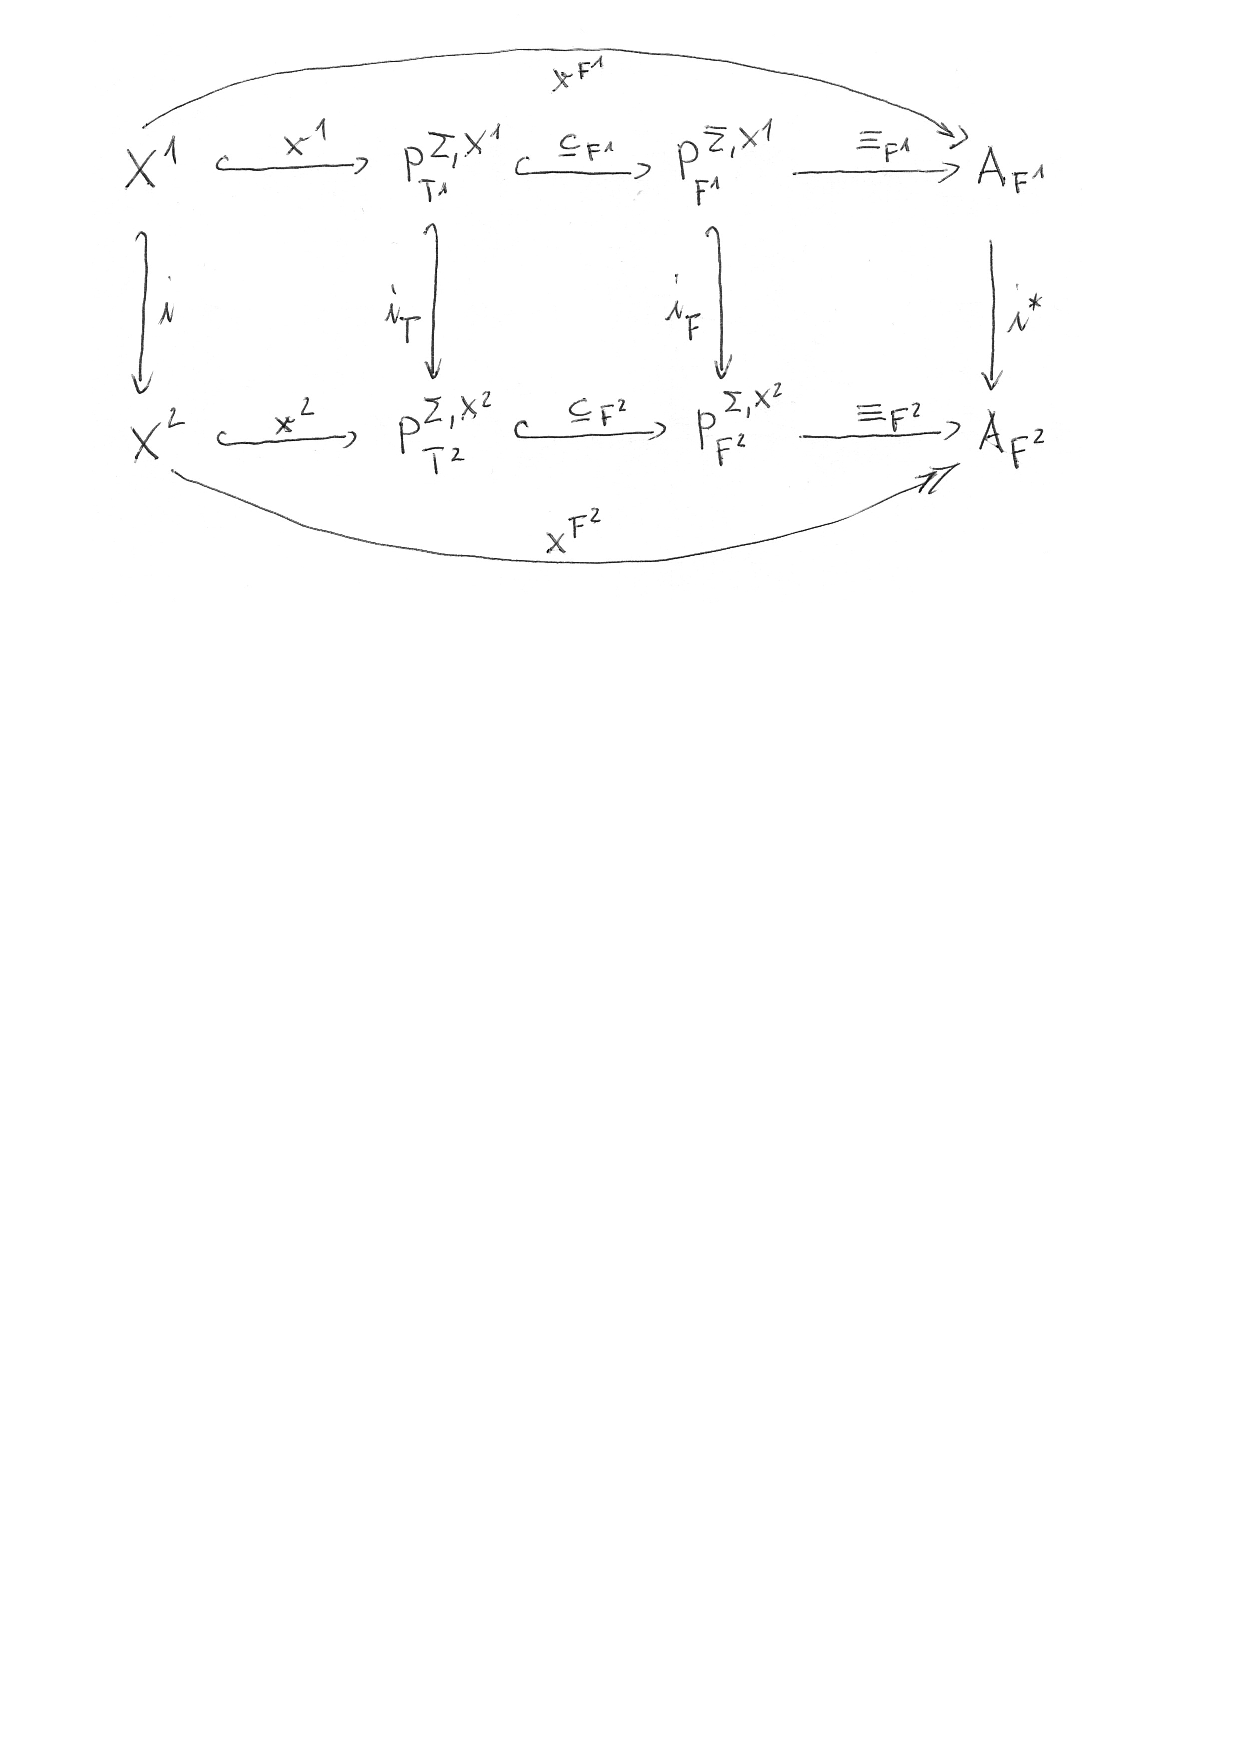
\includegraphics[scale=0.5]{Abbildungen/180}\caption{Sub-Präsentationen}
\end{figure}

\paragraph{\defi 181 Erweiterte Auswertung}
Gegeben $h: X \rightarrow A$ Variablenzuweisung. $F(h) = (X,(F(h)_s)_{s \in S \cup \{\epsilon\}}$ (Syntaktische Präsentation des geschlossenen Sub-Systems von $A$, welches generiert wurde durch $h(X)$) ist die kleinste Menge von Formeln definiert durch
\begin{enumerate}
\item $(F(h)_s = P(h)_s)_{s \in S}$ und 
\item $f(x) \in F(h)_\epsilon$, wenn $f \in O_{w, \epsilon}$, $f \in P(h)^w$, und $f^A$ ist definiert für $(h*)^w(x)$
\end{enumerate}

\paragraph{\coro 182 Erweiterte Auswertung und Homos}
$k: A \rightarrow B$ ist Homo und $h: X \rightarrow A$ Variablenzuweisung $\implies $ $F(h) \subseteq F(k \circ h)$

\paragraph{\coro 183 Syntaktische Präsentation für ein System}
$\mathbf{A}_{F(id_A)} \approx A$, wobei $id_A: (A_s)_{s \in S} \rightarrow A$ ist die identische Variablenzuweisung definiert durch $a \mapsto a$ für alle $a \in (A_s)_{s \in S*}$

\paragraph{\coro 184 Syntaktische Präsentation von Epis}
$e: B \twoheadrightarrow C$ ist epi $\implies \mathbf{A}_{F(e)} \approx C$ und $\approx \circ x^{F(e)} = e$


\section{Approximation}
\subsection{kommt nix}
\subsection{kommt nix}
\subsection{Pushout und Pullback}

\paragraph{\defi 206 Span, Co-Span}
In einer Kategorie $\mathcal{C}$: \\Span ist ein Paar $(p,q)$ von Morphismen mit der selben Domain. \\
Co-Span ist so ein paar mit der selben Co-Domain. \\ 
 \emph{Notiz: Span ist ein Diagramm von Graphen $\bullet \leftarrow \bullet \rightarrow \bullet$ und ein Co-Span \\ ist ein Diagramm von $\bullet \rightarrow  \bullet \leftarrow \bullet$ }

\begin{multicols}{2}
\columnseprule1pt

\textbf{\underline{Pushout}} 

\textbf{\defi 207 Pushout} \\
Ein Pushout eines Span $(P: a \nach b, q: a \nach c)$ ist ein Paar von Morphismen $(p^*: c \nach d, q^*: b \nach d)$, so dass $(p^*, q^*, p^* \circ q = q^* \circ p)$ ist der Co-Limit des Span. \\
\emph{Notiz: Zwei Morphismen $p^*$ und $q^*$ Charakterisieren den Co-Limes, der dritte $p^* \circ q = q^* \circ p$ kann von der Co-Cone-Eigenschaft abgeleitet werden.}

\textbf{\coro 208 Pushout Komposition} \\
\ref{fig:208} ist kommutatives Diagramm und $(1)$ ist Pushout, dann $(2)$ ist Pushout $\Leftrightarrow$ das ganze Diagramm $(1)+(2)$ ist ein Pushout.




\columnbreak

\textbf{\underline{Pullback}} 

\textbf{\defi 216 Pullback} \\
Ein Pullback eines Co-Span $(p: b \nach a, q: c \nach a)$ ist ein Paar von Morphismen $(p^*: d \nach c, q^*: d \nach b)$, so dass $p^*,q^*, q \circ p^* = p \circ q^*$ ist der Limit des Co-Span.

\end{multicols}

\begin{figure}[h]
\centering
\subfigure[Pushout\label{fig:208}]{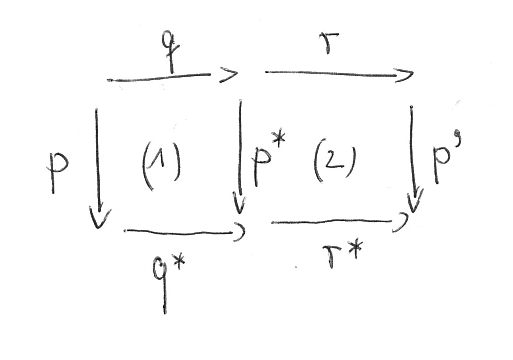
\includegraphics[width=0.21\textwidth]{Abbildungen/208}} \qquad \qquad \qquad
\subfigure[Pullback\label{fig:217}]{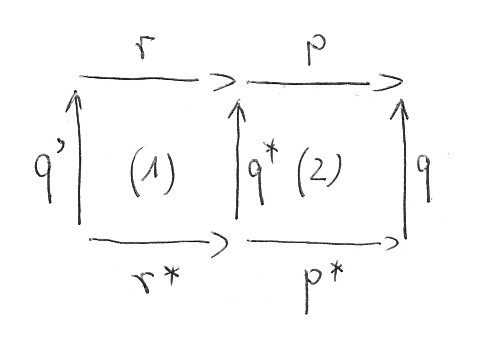
\includegraphics[width=0.20\textwidth]{Abbildungen/217}}
\caption{Definitionen}
\end{figure}


\begin{multicols}{2}
\columnseprule1pt

\textbf{\underline{Pushout}} 

\textbf{\coro 209 Pushout Dekomposition} \\
In einer Kategorie, in welcher jeder Span ein Pushout hat kann der Pushout ($p^*, (r \circ q)^*$) des Span $(p, r \circ q)$ dekomponiert werden in zwei Produkte 
\begin{enumerate}
\item $(p' q^*)$ von $(p,q)$ und 
\item $(p^*, r^*)$ von $(p', r)$, so dass \\ $(r \circ q)^* = r^* \circ q*$
\end{enumerate}

\textbf{\coro 210 Pushouts bewahren Epis} \\
$(p^*, q^*)$ ist Pushout $(p,q)$ und $p$ ist Epi.\\
$\implies p^*$ ist epi.


\columnbreak

\textbf{\underline{Pullback}} 

\textbf{\prop 151 Binäres Co-Produkt in \syssig} \\
Das variante System $A + B$ ist das Co-Produkt der zwei Systeme $A$ und $B$.

\end{multicols}

\begin{figure}[h]
\centering
\subfigure[Pushout\label{fig:209}]{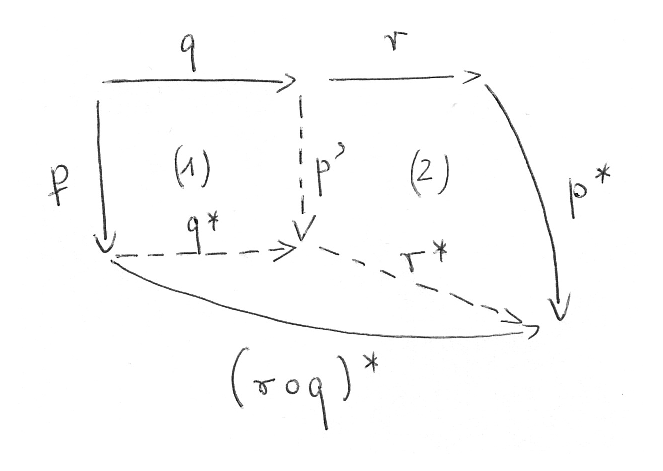
\includegraphics[width=0.22\textwidth]{Abbildungen/209}} \qquad \qquad \qquad
\subfigure[Pullback\label{fig:todo}]{
\includegraphics[width=0.22\textwidth]{Abbildungen/todo}}
\caption{Dekomposition}
\end{figure}

\begin{figure}[h]
\centering
\subfigure[Pushouts und Epis\label{fig:210}]{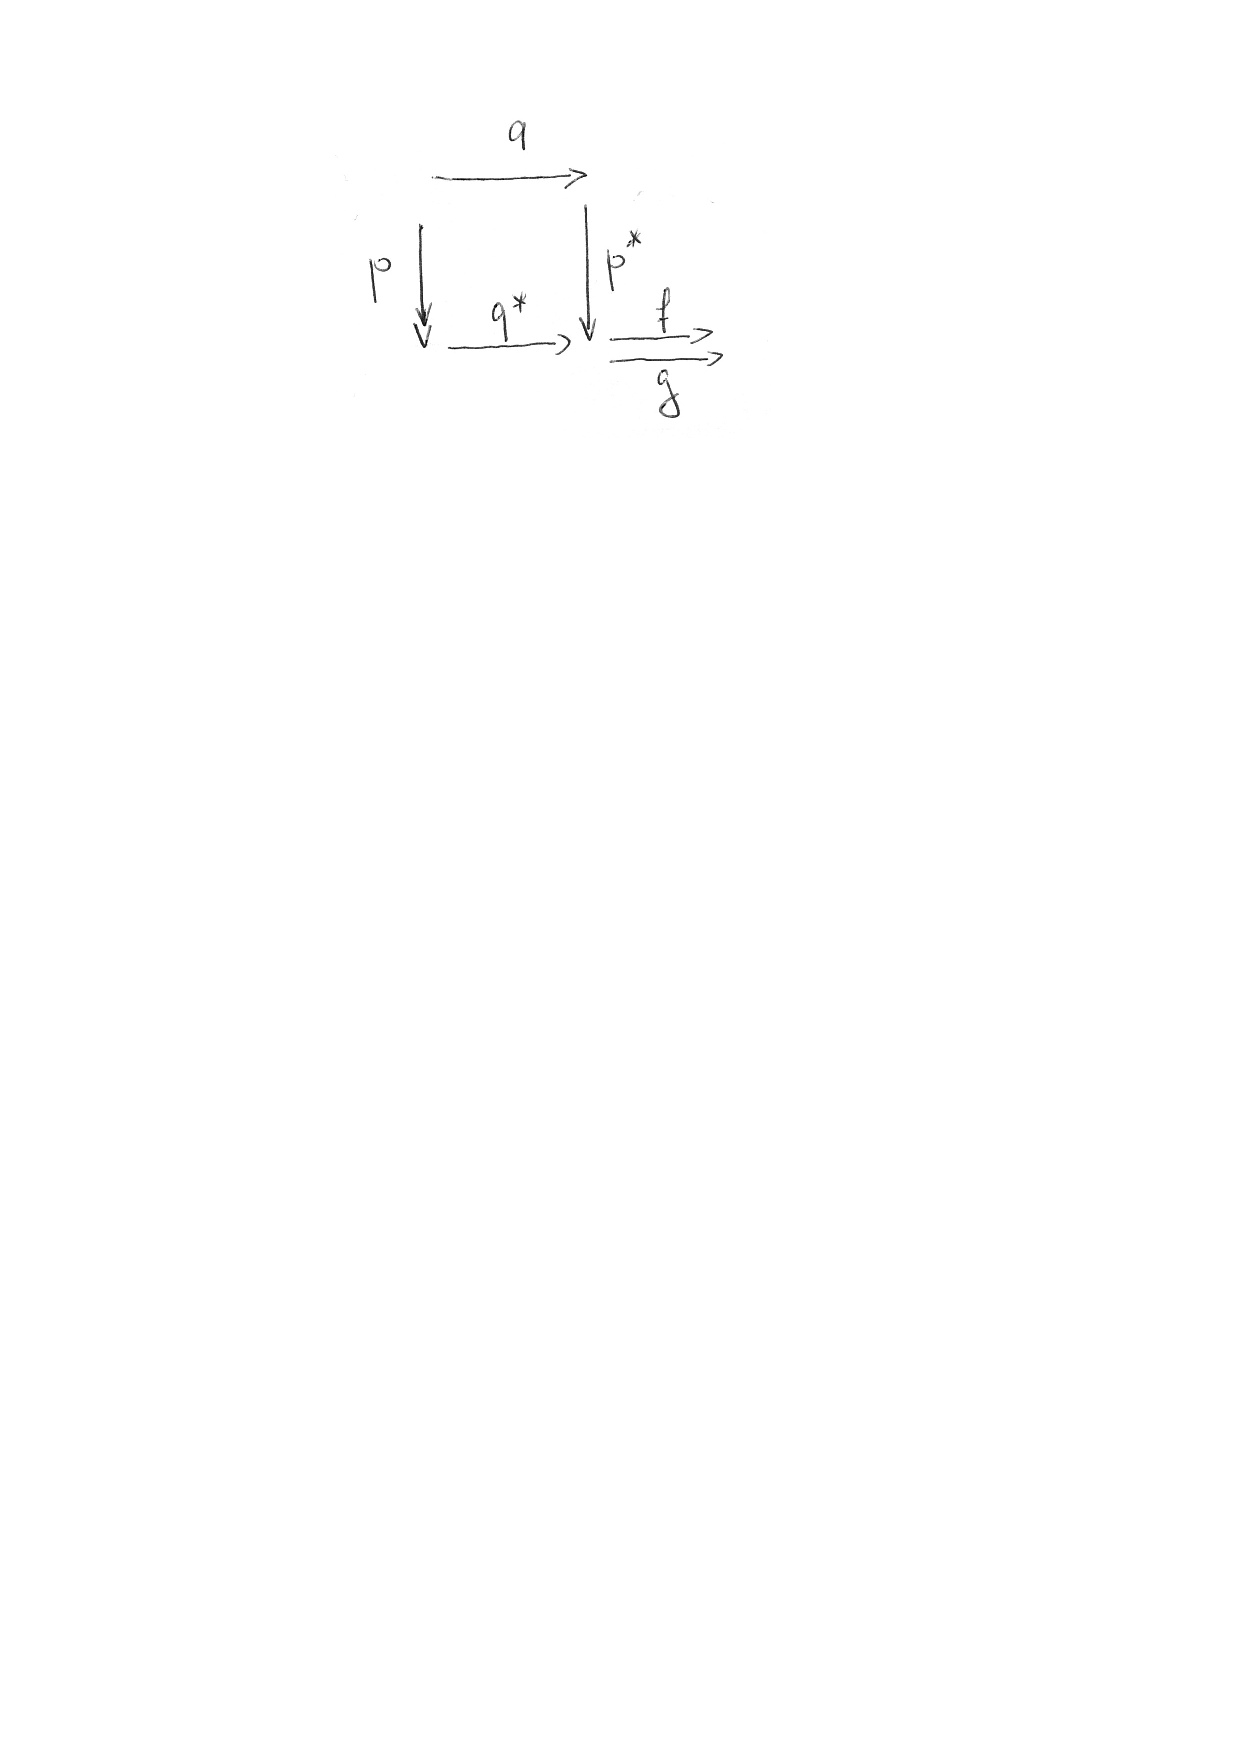
\includegraphics[width=0.22\textwidth]{Abbildungen/210}} \qquad \qquad \qquad
\subfigure[Pullback\label{fig:todo}]{
\includegraphics[width=0.22\textwidth]{Abbildungen/todo}}
\caption{Pushouts und Pullbacks}
\end{figure}

\newpage 

\begin{multicols}{2}
\columnseprule1pt

\textbf{\underline{Pushout}} 

\textbf{\prop 211 Pushouts bewahren extremale Epis} \\
Die zugrundeliegende Kategorie $(\mathcal{C})$ hat ein $(\mathcal{E}^x, \mathcal{M})$, $(p^*, q^*)$ ist Pushout von $(p,q)$ und $p$ ist extremal Epi $\implies$ $p^*$ ist extremal Epi.

\textbf{\prop 212 Pushouts bewahren Sektionen} \\
$(p^*, q^*)$ ist Pushout von $(p,q)$ und $p$ ist Sektion $\implies $ $p^*$ ist Sektion.

\textbf{\coro 213 Abgeleitete Pushouts} \\
$(p^*, q^*)$ ist Pushout von $(p,q)$, wobei $p$ Sektion $\implies$ $\left ( q, (p^*)^{-1} \right )$ ist Pushout von $(q^*, p^{-1})$, wenn wir $(p^*)^{-1}$ als das eindeutige $u$ in Prop 212 wählen.

\columnbreak

\textbf{\underline{Pullback}} 

\textbf{\prop 151 Binäres Co-Produkt in \syssig} \\
Das variante System $A + B$ ist das Co-Produkt der zwei Systeme $A$ und $B$.

\end{multicols}


\begin{figure}[h]
\centering
\subfigure[Pushouts und extremal Epi\label{fig:211}]{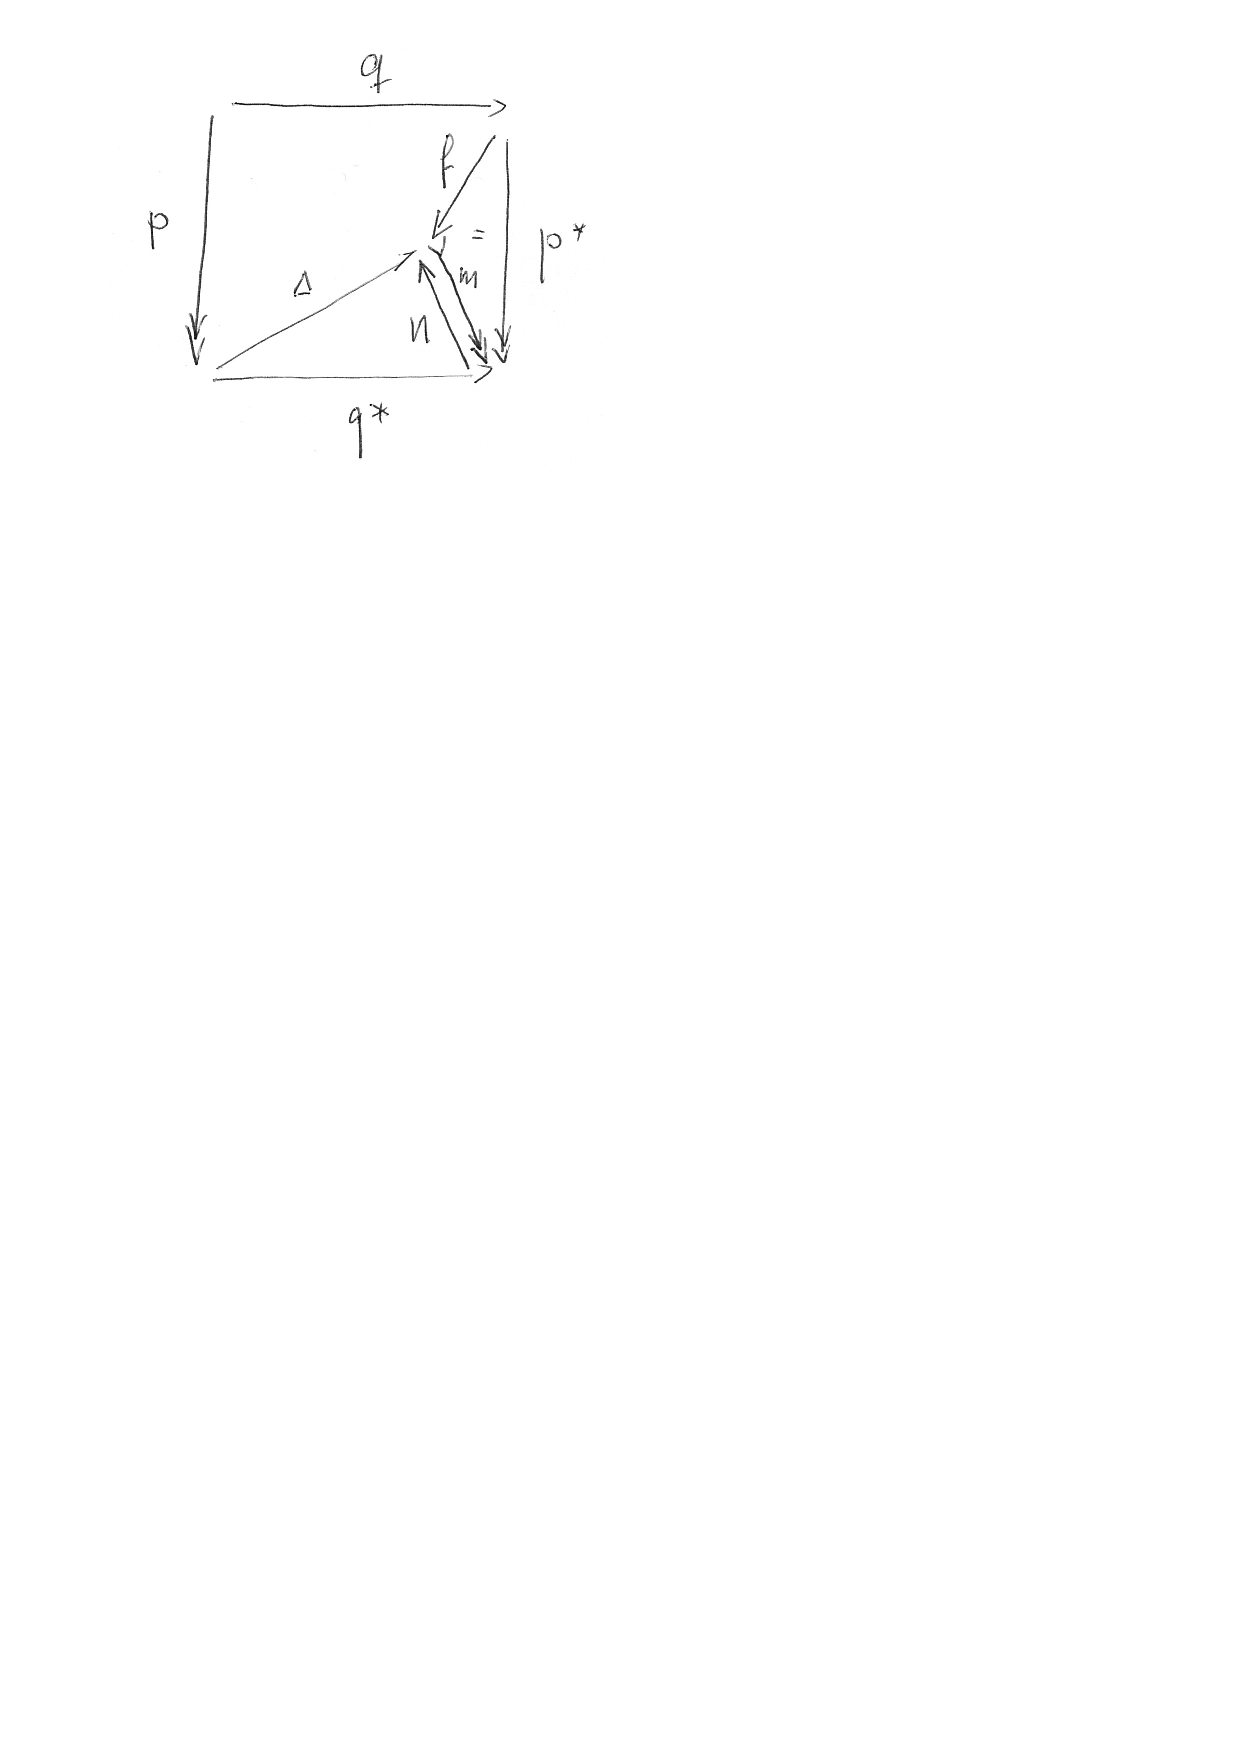
\includegraphics[width=0.22\textwidth]{Abbildungen/211}} \qquad \qquad \qquad
\subfigure[Pullback\label{fig:todo}]{
\includegraphics[width=0.22\textwidth]{Abbildungen/todo}}
\caption{Pushouts und Pullbacks}
\end{figure}

\begin{figure}[h]
\centering
\subfigure[Pushouts und extremal Epi\label{fig:212}]{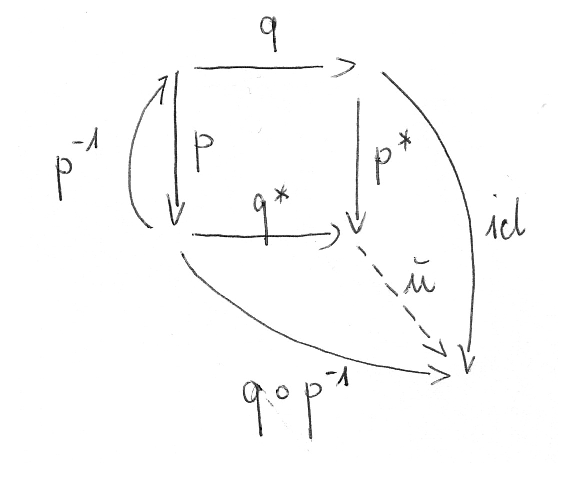
\includegraphics[width=0.22\textwidth]{Abbildungen/212}} \qquad \qquad \qquad
\subfigure[Pullback\label{fig:todo}]{
\includegraphics[width=0.22\textwidth]{Abbildungen/todo}}
\caption{Pushouts und Pullbacks}
\end{figure}
\newpage 

\begin{multicols}{2}
\columnseprule1pt

\textbf{\underline{Pushout}} 

\textbf{\coro 214 Pushouts bewahren Isomorphismen} \\
$(p^*, q^*)$ ist Pushout von $(p,q)$ und $p$ Iso $\implies$ $p^*$ ist Iso.

\textbf{\prop 215 Spezielle Pushouts in $Sys(\Sigma)$} \\
Wenn $(p:A\rightarrowtail B,q:A\rightarrowtail C)$ span extremaler Monos  in $\mathsf{Sys}(\Sigma)$, kann der pushout $(p^{*}:C\rightarrowtail D,q^{*}:B\rightarrowtail D)$
wie folgt konstruiert werden. Obda. Angenommen, dass $A_{s}$, $B_{s}$, und $C_{s}$ paarweise disjunkt sind, jede Sorte  $s$:

\begin{align*}
\textrm{\emph{(i)} } & \forall \, s\in S: \\ & D_{s}=A_{s}\cup\left(B_{s}-p(A_{s})\right)\cup\left(C_{s}-q(A_{s})\right)\\
\textrm{\emph{(ii)} } & \forall \, s \in S\textrm{ and }c\in C_{s}: \\ &  p_{s}^{*}(c)=\begin{cases}
a & c=q(a)\\
c & \textrm{otherwise} 
\end{cases}\\
\textrm{\emph{(iii)} } &  \forall \, s\in S\textrm{ and }b\in B_{s}: \\ & q^{*}(b)=\begin{cases}
a & b=q(a)\\
b & \textrm{otherwise}
\end{cases}\\
\textrm{\emph{(iv)} } &  \forall \, f \in O_{w,v}:\\ & f^{D}(x)=\begin{cases}
\left(p^{*}\right)^{v}(y_{C}) \, \, \, \, \, \,  \, \,  f^{C}(x_{C})=y_{C}\\
\, \, \, \, \, \,  \, \, \, \, \, \, \, \,  \, \, \, \, \, \, \, \,  \, \, \, \, \,  \textrm{ and }f^{C}(x_{C})=y_{C}\\
\left(q^{*}\right)^{v}(y_{B}) \, \, \, \, \, \,    \textrm{if }x=\left(q^{*}\right)^{w}(x_{B})\\
\, \, \, \, \, \,  \, \, \, \, \, \, \, \,  \, \, \, \, \, \, \, \,  \, \, \, \, \, \textrm{ and }f^{B}(x_{B})=y_{B}\\
\textrm{undefined} \, \, \, \, \, \,  \, \,  \textrm{otherwise}
\end{cases}
\end{align*}



\columnbreak

\textbf{\underline{Pullback}} 

\textbf{\prop 151 Binäres Co-Produkt in \syssig} \\
Das variante System $A + B$ ist das Co-Produkt der zwei Systeme $A$ und $B$.

\end{multicols}



\newpage

\section{Varietät}

\subsection{Atomare Axiome}

\paragraph{\defi 238 Atomares Axiom und Lösung}
Gegeben: $\Sigma = (S,O)$, atomares Axiom $a = (X, f)$ besteht aus einer endlichen Variablenmenge $X$ und einer Formel $f \in F^{\Sigma, X}$. \\
Eine Variablenzuweisung $h: X \rightarrow B$ in ein $\Sigma$-System B löst das Axiom $A = (X, f)$, wenn es einen \homo $h^*: \mathbf{A}_a \rightarrow B$ gibt, so dass $h^* \circ x^a = h$. \\
Wenn $h$ eine Lösung ist, schreiben wir $h \models a$

\paragraph{\prop 239 Homomorphismus und Lösung}

$h: X \nach B$ ist Lösung von atomarem Axiom $a = (X,f)$ in $B$ und $k: B \rightarrow C$ ist ein \homo $\implies k \circ h$ löst $a$ in $C$, d.h. $k \circ h \models a$.


\paragraph{\defi 240 Gültigkeit atomarer Axiome}

$a= (X,f) $ ist gültig in einem algebraischen System $B$ ($B \models a$), wenn jede Variablenzuweisung $h: X \nach B$ $a$ löst, d.h. \\
$B \models a$ wenn $\forall \, h: X \nach B :: h \models a$.

\paragraph{\prop 241 Gültigkeit ist abstrakt}
Wenn $a$ atomares Axiom ist, $B \models a$, und $B \approx B' \implies B' \models a$.  

\paragraph{\defi 242 Gefülltes algebraisches System}
Ein  algebraisches System $B$ ist gefüllt, wenn jede Trägermenge von $B$ nicht leer ist (d.h. 
$B_s \neq \emptyset$ für alle $s \in S$) \\ $S' \subseteq S \implies$ $B$ ist '$S'$-gefüllt', wenn $B_{s} \neq \emptyset \,$ für alle $s \in S'$.  

\paragraph{\prop 244 Gültigkeit in Produkten}
$a$ atomres Axiom, $I$ indizierte Menge. \\$(B_i \models a)_{i \in I} \implies \Pi(B_i)_{i \in I} \models a$


\paragraph{\prop 245 Gültigkeit in extremalen Subsystem}
$a$ atomares Axiom, $i: C \rightarrowtail B$ extremaler Mono, $B \models a \implies C \models a$

\paragraph{\defi 246: Homomorphe Bilder }
Algebraisches System $C$ ist homomorphes Bild eines Systems $B$, wenn es einen surjektiven Homomorphismus $q: B \twoheadrightarrow C$ gibt.

\emph{(Notiz: Homomorphes Bild ist Spezialfall von Epi (Vgl. Prop 80) (Bedenke: Wenn surjektiv, dann Epi. Umgekehrt nicht)) }


\paragraph{\prop 247: Gültigkeit in homomorphen Bildern}
$B \models a$, $C$ homomorphes Bild von $B$, d.h. Es gibt einen surjektiven \homo $q: B \twoheadrightarrow C \implies C \models a$

\emph{Notiz CT aus der Vorlesung: Wenn $C \models a$ und $h: B \rightarrowtail C$ injektiver Homo $\implies$: $B \models a$}

\paragraph{\coro 248: Gültigkeit in Produktkomponenten}
$a = (X,f)$ atomares Axiom und $S_X \subseteq S$ (Teilmenge der Sorten für welche $a$ Variablen hat), d.h. $s \in S_X \Leftrightarrow X_s \neq \emptyset$.
$\Pi (B_i)_{i \in I} \models a$ und $(B_{i,s} \neq \emptyset)_{i \in I, s \in S_X}$ ('$S_X$' gefüllt) \\
$\implies  B_i \models a \, \, \forall \,  i \in I $ (jede Komponente des Produktes erfüllt das Axiom).

\paragraph{\lem 249: Variablenzuweisung in approximierte Systeme}
(ausgelassen)

\paragraph{\prop 250: Gültigkeit in approximierte Systemen}
(ausgelassen)


\subsection{Atomare Spezifikationen}

\paragraph{\defi 251: Atomare Spezifikation, Varietäten} 
Atomare Spezifikation \\ $ASpec = (\Sigma, \Phi)$ besteht aus einer Signatur $\Sigma$ und einer Menge von atomaren Axiomen $\Phi$ wrt. $\Sigma$.
$B \in Sys(\Sigma) $ erfüllt die Spezifikation (geschrieben: $B \models ASpec$), wenn $B \models a$ für alle $a \in \Phi$. \\
Die volle Subkategorie von \syssig, welches alle Systeme beinhaltet, die die Spezifikation $ASpec = (\Sigma, \Phi)$ erfüllen, wird bezeichnet als Sys($ASpec$) oder Sys$(\Phi)$. \\
Eine volle Subkategorie $\mathbb{K}$ aller $\Sigma$-Systeme wird eine Varietät genannt, wenn es eine atomare Spezifikation ($\Sigma, \Phi$) gibt, so dass $\mathbb{K} = Sys(\Phi)$


\paragraph{\prop 252: Varietäten sind abstrakt} 
Jede Varietät ist isomorph-geschlossen. Siehe Defi 253.

\paragraph{\defi 253: Bündel atomarer Axiome, Lösungen} 
Ein Bündel $\mathcal{B}$ atomarer Axiome mit den selben Variablenmengen $X$ ist eine syntaktische Präsentation $\mathcal{B} = (X, F \subseteq F^{\Sigma, X})$.
$C$ erfüllt ein Bündel (geschrieben: $C \models \mathcal{B}$), wenn jede Variablenzuweisung $h: X \nach C$ erweitert werden kann auf einen \homo $h^*: \mathbf{A}_\mathcal{B} \nach C$, so dass $h^* \circ^\mathcal{B} = h$


\paragraph{\lem 254: Bündel definieren Co-Limiten} 
(ausgelassen)

\paragraph{\prop 255: Bündel atomarer Axiome} 

$(a_i)_{i \in I}$ ist Familie atomarer Axiome mit den selben Variablenmengen $X$, d.h. $a_i = (X, f_i)$ für alle $i \in I$ \\ 
$\implies C $ erfüllt alle Axiome $((C \models a_i )_{i \in I})$ $\Leftrightarrow$ $C$ erfüllt das Bündel $\mathcal{B} = (X, \{f_i:: i \in I \})$, d.h. $C \models \mathcal{B}$ 

\paragraph{\lem 256: Co-well-powered Basis} 
\syssig its co-well-powered.


\paragraph{\coro 257: Varietäten sind episch-reflektive Subkategorien}
Jede Varietät $\mathbb{K} \subseteq Sys(\Sigma)$ ist episch-reflektive Subkategorie von \syssig.

\paragraph{Theorem 258: Birkhoffs Charakterisierung}
Eine volle Unterkategorie $\mathbb{K}$ von \syssig ist eine Varietät $\Leftrightarrow $ $\mathbb{K}$ ist geschlossen bis auf Produkte, extremale Subobjekte, homomorphe Bilder und approximierte Systeme. 
 
 
\newpage  
\subsection{Spezifikationsproblem und einfache Lösung}

\paragraph{\defi 259: Spezifikationsproblem, einfache Lösung}
Ein Spezifikationsproblem ist gegeben durch eine Signatur $\Sigma$ und entweder 
\begin{enumerate}
\item Ein $\Sigma$-System K oder
\item Eine volle und isomorph-geschlossene Subkategorie $\mathbb{K} \subseteq Sys(\Sigma)$ 
\end{enumerate}
Eine einfache Lösung für das Spezifikationsproblem ist eine atomare Spezifikation $ASpec = (\Sigma, \Phi)$, so dass 
\begin{enumerate}
\item $K$ ist initial in $Sys(ASpec)$ oder
\item $Sys(ASpec) = \mathbb{K}$
\end{enumerate}


\paragraph{\coro 261: Reflektion des initialen Objektes}
$\mathcal{D}$ relflektive Subkategorie von $\mathcal{C}$, $\mathcal{C}$ hat initiales Objekt $\mathcal{I}$ $\implies$ Reflektion $\mathcal{I}_{\mathcal{D}}$ von $\mathcal{I}$ ist initial in $\mathcal{D}$

\paragraph{\coro 262: Spezifizierbare Systeme}
Eine Spezifikationsproblem $K \in Sys(\Sigma)$ vom Typ 1. (siehe Defi 259 1.) ist lösbar $\Leftrightarrow$ $K$ ist generiert durch seine Operationen, d.h. $K = \left\lceil i\left(\emptyset^{\Sigma}\right)\right\rceil ^{c}$, wobei $i: \emptyset^\Sigma \rightarrow K$ ist der eindeutige Homomorphismus vom initialen Objekt nach $K$.

\section{Quasi Varietäten}

\subsection{Horn-Typ Axiome}

\paragraph{\defi 264: Hornaxiom}
Hornaxiom $a = (X, P \subseteq F^{\Sigma,X}, c \in F^{\Sigma,X})$ \\
$X$ ist endliche Variablenmenge, $P$ (Prämisse) endliche syntaktische Präsentation, $c \in F^{\Sigma,X}$ Formel (Konklusion).

\paragraph{\defi 265: Gültigkeit von Hormaxiomen}
Hormaxiom $a = (X, P, c)$ ist gültig in einem algebraischen System $B$ $(B \models a)$, wenn jeder Morphismus \\ $h: \mathbf{A}_P \nach B$ erweitert werden kann zu einem \homo \\ $h^*: \mathbf{A}_{c^P} \nach B$, so dass $h^* \circ x_{p}^c = h$, wobei $c^p = (X,P \cup \{c\})$ und $x^{c}_P: \mathbf{A}_P \nach \mathbf{A}_{c^P}$ ist der eindeutige \homo, der $x_P^c \circ x^P = x^{c^P}$ erfüllt.

\paragraph{\prop 266: Gültigkeit ist abstrakt}
$a = (X, P, c)$ Hornaxiom, $B \models a$, $B \approx B'$ $\implies$ $B' \models a$.


\paragraph{\prop 267: Gültigkeit Produkt und Subsystem}
$a = (X, P, c)$ Hornaxiom
\begin{enumerate}
\item $I$ Indexmenge, $(B_i \models a)_{i \in I}$ $\implies$ $\Pi (B_i)_{i \in I} \models a$
\item $i: C \rightarrowtail B$ extremal Mono, $B \models a$ $\implies $ $C \models a$
\end{enumerate}

\paragraph{\lem 268: \homos in approximierte Systeme}
$(I, \leq)$ gerichtete Indexmenge $\mathcal{H} = \left( (B^I)_{I \in I} (k^{i,j}: B^i \nach B^j)_{i,j \in I, i \leq j} \right)$ approximierte Situation \\ mit approximierende System 
$\left(\mathcal{H}{}^{\bullet},\left(i^{\bullet}:B^{i}\rightarrow\mathcal{H}{}^{\bullet}\right)_{i\in I}\right)$,
\\ $F=\left(X,F\subseteq F^{\Sigma,X}\right)$ endliche syntaktische Präsentation, \\
 $m:\mathbf{A}_{F}\rightarrow\mathcal{H}{}^{\bullet}$ homo, \\
$\implies$ es gibt $j\in I$ und ein Homo $m':\mathbf{A}_{F}\rightarrow B^{j}$, so dass  $m=j^{\bullet}\circ m'$.


\paragraph{\prop 269: Gültigkeit in  approximierten Systeme}
$(I, \leq)$ ist eine gerichtete, partiell geordnete Indexmenge und $\mathcal{H} = \left( (B^i)_{i \in I}, (k^{i,j}: B^i \nach B^j)_{i,j \in I, i \leq j} \right)$ eine approximierende Situation, so dass $(B^i \models a)_{i \in I}$ für ein Hornaxiom $a$ \\
$\implies $ $a$ ist gültig im approximierten System $\mathcal{H}^\bullet$, d.h. $\mathcal{H}^\bullet \models a$

\subsection{Horntyp Spezifikation}

\paragraph{\defi 270: Horn-Spezifikation}
Ein Horntyp-Spezifikation $HSpec = (\Sigma, \Phi)$ besteht aus einer Signatur $\Sigma$ und einer Menge an Hornaxiomen $\Phi$ wrt. to $\Sigma$. \\
Algebraisches System $B \in Sys(\Sigma)$ erfüllt die Spezifikation $(B \models HSpec$  oder $B \models \Phi)$, wenn $B \models a$ für alle $a \in \Phi$.  \\
Die volle Subkategorie von $Sys(\Sigma)$, welche alle Systeme beinhaltet, die die Spezifikation $HSpec = (\Sigma, \Phi)$ 
erfüllen, wird bezeichnet als $Sys(HSpec)$ oder $Sys(\Phi)$. \\
Eine volle Subkategorie $\mathbb{K}$ aller $\Sigma$-Systeme wird Hornklasse genannt, wenn es eine Hornspezifikation $HSpec = (\Sigma, \Phi)$ gibt, so dass $\mathbb{K} = Sys(HSpec)$.

\paragraph{\prop 271: Hornklassen sind abstrakt}
Jede Hornklasse ist isomorph-geschlossen.

\paragraph{\defi 272: Bündel von Hornaxiomen, Lösung}
Ein \emph{Bündel }$\mathcal{B}=\left(X,P\subseteq F^{\Sigma,X},C\subseteq F^{\Sigma,X}\right)$\emph{
von Hormaxiomen} mit der gleichen endlichen Variablenmenge  $X$ \emph{und}
der gleichen endlichen Menge  von prämissen $P$ besteht aus zwei syntaktischen Präsentationen
$P$ und $C$. \\
Die syntaktische Präsentation für Prämisse und Konklusion wird bezeichnet als $C^{P}=(X,P\cup C)$. \\
Der eindeutige Epimorphismus, der $x_{P}^{C}\circ x^{P}=x^{C^{P}}$ erfüllt, wird bezeichnet als  $x_{P}^{C}:\mathbf{A}_{P}\rightarrow\mathbf{A}_{C^{P}}$. \\
Ein algebraisches System $D$ erfüllt ein Bündel  ($D\models\mathcal{B}$),
wenn jeder Homo $h:\mathbf{A}_{P}\rightarrow D$ erweitert werden kann
zu einem Homo $h^{*}:\mathbf{A}_{C^{P}}\rightarrow C$, so dass
$h^{*}\circ x_{P}^{C}=h$.

\paragraph{\lem 273: Bündel definieren Co-Limiten}
$\left(a_{i}=\left(X,P,c_{i}\right)\right)_{i\in I}$ ist eine Familie von Hornaxiomen, mit der selben Variablenmenge
$X$ und der selben Menge von Prämissen $P$ und dessen Bündel $\mathcal{B}$ \\ 
$\implies$  $\mathbf{A}_{\mathcal{B}}$
ist Co-Limit von $\left(x^{c_{i}^{P}}:\mathbf{A}_{P}\rightarrow\mathbf{A}_{c_{i}^{P}}\right)_{i\in I}$

\paragraph{\lem 274: Bündel von Hornaxiomen}
Wenn $(a_i)_{i \in I}$ ist Familie von Hornaxiomen mit der gleichen Variablenmenge $X$ und der gleichen Menge von Prämissen, das heißt $a_i = (X, P, c_i)$ für alle $i \in I$ \\
dann $\implies$ ein algebraisches System $D$ erfüllt alle Axiome, d.h. $(D \models a_i)_{i \in I}$ $\Leftrightarrow$ $D$ erfüllt das Bündel $\mathcal{B} = (X, P, \{c_i:: i \in I\})$, d.h. $D \models \mathcal{B}$

\paragraph{Theorem 276: Charakterisierung von Hornklassen}
Eine volle Subkategorie $\mathbb{K}$ von $Sys(\Sigma)$ ist eine Hornklasse $\Leftrightarrow$ $\mathbb{K}$ ist geschlossen bis auf Produkte, extremale Subobjekte und approximierte Systeme.



